% Source printed pp. 16-28, entire Section 1.3.
\section{函子观点}\label{src:1.3}
\begin{epigraph}
数学对象由它们与同类的所有其他对象之间的关系网络所决定, 也通过这一网络得到理解.
\epigraphauthor{Barry Mazur~\cite{Maz08}}
\end{epigraph}
定义一个\newterm{模函子}{moduli functor}, 需要明确: 
\begin{enumerate}[(1)]
\item 对象的族; 
\item 两个对象族在什么情形下等价; 以及
\item 对象族如何沿态射拉回.
\end{enumerate}
在代数范畴中, 这些数据汇集为一个反变函子
\begin{equation}\label{src:1.3.1}
F:\Sch\longrightarrow\Sets,\qquad S\longmapsto\{S\text{ 上的对象族}\},
\end{equation}
其中, 对映射 $f:S\to T$, $F(f):F(T)\to F(S)$ 给出从 $T$ 上的族到 $S$ 上的族的拉回映射, 有时简记为 $f^*$.(要成为函子, 拉回映射必须与复合相容: 对映射 $f:S\to T$ 和 $g:T\to U$, 有 $F(g\circ f)=F(f)\circ F(g)$.)

\subsection{族的重要性}\label{src:1.3.1-subsection}
通过族, 我们能够精确表述模空间 $M$. 空间 $S$ 上的对象族 $\mathcal C$ 定义一个集合映射
\begin{equation}\label{src:1.3.2}
S\longrightarrow M,\qquad s\longmapsto[\mathcal C_s],
\end{equation}
其中, 纤维 $[\mathcal C_s]\in M$ 是 $\mathcal C$ 沿包含映射 $\{s\}\hookrightarrow S$ 的拉回. 在拓扑范畴(相应地, 在代数范畴)中, 我们希望映射 $S\to M$ 连续(相应地, 为代数映射). 理想情况下, $S$ 上的族与态射 $S\to M$ 一一对应; 换言之, 空间 $M$ 表出~\eqref{src:1.3.1}~中的函子 $F$. 如果如此, 我们称 $M$ 为细模空间; 不过很快就会看到, 这往往是过高的奢望.

通过族来定义模空间有如下优点: 
\begin{itemize}
\item 可以赋予模集合 $M$ 更丰富的结构. 要给 $M$ 赋予拓扑, 我们规定: 子集 $U\subseteq M$ 为开集, 当且仅当对每个 $S$ 上的对象族 $\mathcal C$, 集合 $\{s\in S\mid[\mathcal C_s]\in U\}$ 都是 $S$ 的开子集. $M$ 上的整体函数 $f$ 可以定义为一组数据: 对每个 $S$ 上的族 $\mathcal X$, 给定 $S$ 上的整体函数 $f_{\mathcal X}$, 且这些函数彼此相容.
\item 当 $M$ 为细模空间时, 恒等映射 $\mathrm{id}:M\to M$ 对应于模空间 $M$ 上的一个对象族 $\mathcal U$. 这就是\newterm{万有族}{universal family}: 对任意其他 $S$ 上的族 $\mathcal C$, 存在唯一态射 $S\to M$(其集合映射由~\eqref{src:1.3.2}~给出), 使万有族 $\mathcal U$ 拉回为 $\mathcal C$.
\end{itemize}
这无疑是抽象程度上的巨大飞跃!而且看起来我们似乎只是让事情更难了: 我们不再通过指定空间的点, 拓扑以及可能具有的复结构或代数结构来引入空间, 而必须指定大量范畴数据. 然而, 实践中通常很容易定义性质良好的族的概念. Yoneda 引理(\bookref{1.3.12})确立了这种观点的转变: 到一个空间的映射所组成的函子, 唯一决定该空间.

\begin{example}[带标号三角形的族]\label{src:1.3.3}
回到例~\bookref{1.2.8}~中引入的带标号三角形在相似关系下的模, 我们将拓扑空间 $S$ 上的\textit{带标号三角形的族}定义为一个元组 $(\mathcal T,\sigma_1,\sigma_2,\sigma_3)$, 其中 $\mathcal T\to S$ 是一个带有三个截面 $\sigma_i:S\to\mathcal T$ 的纤维丛, 配备连续距离函数 $d:\mathcal T\times_S\mathcal T\to\mathbb R_{\geq0}$. 要求对每个点 $s\in S$, 限制 $d_s:\mathcal T_s\times\mathcal T_s\to\mathbb R_{\geq0}$ 是纤维 $\mathcal T_s$ 上的度量, 并使 $\mathcal T_s$ 等距于一个以 $\sigma_i(s)$ 为顶点的三角形.

称 $S\in\mathsf{Top}$ 上的两个带标号三角形族 $(\mathcal T,(\sigma_i))$ 和 $(\mathcal T',(\sigma_i'))$ \textit{相似}, 是指存在 $S$ 上的同胚 $f:\mathcal T\to\mathcal T'$, 与截面相容(即 $f\circ\sigma_i=\sigma_i'$), 并且对每个 $s\in S$, 所诱导的纤维间映射 $\mathcal T_s\to\mathcal T'_s$ 是三角形的相似变换, 即重新缩放后为等距映射. 给定带标号三角形族 $\mathcal T\to S$ 和连续映射 $S'\to S$, 拉回族定义为集合的纤维积 $\mathcal T\times_S S'$, 配备拉回截面 $\sigma'_i:S'\to\mathcal T'$ 及所继承的距离函数.
\end{example}
\begin{figure}[htbp]
\centering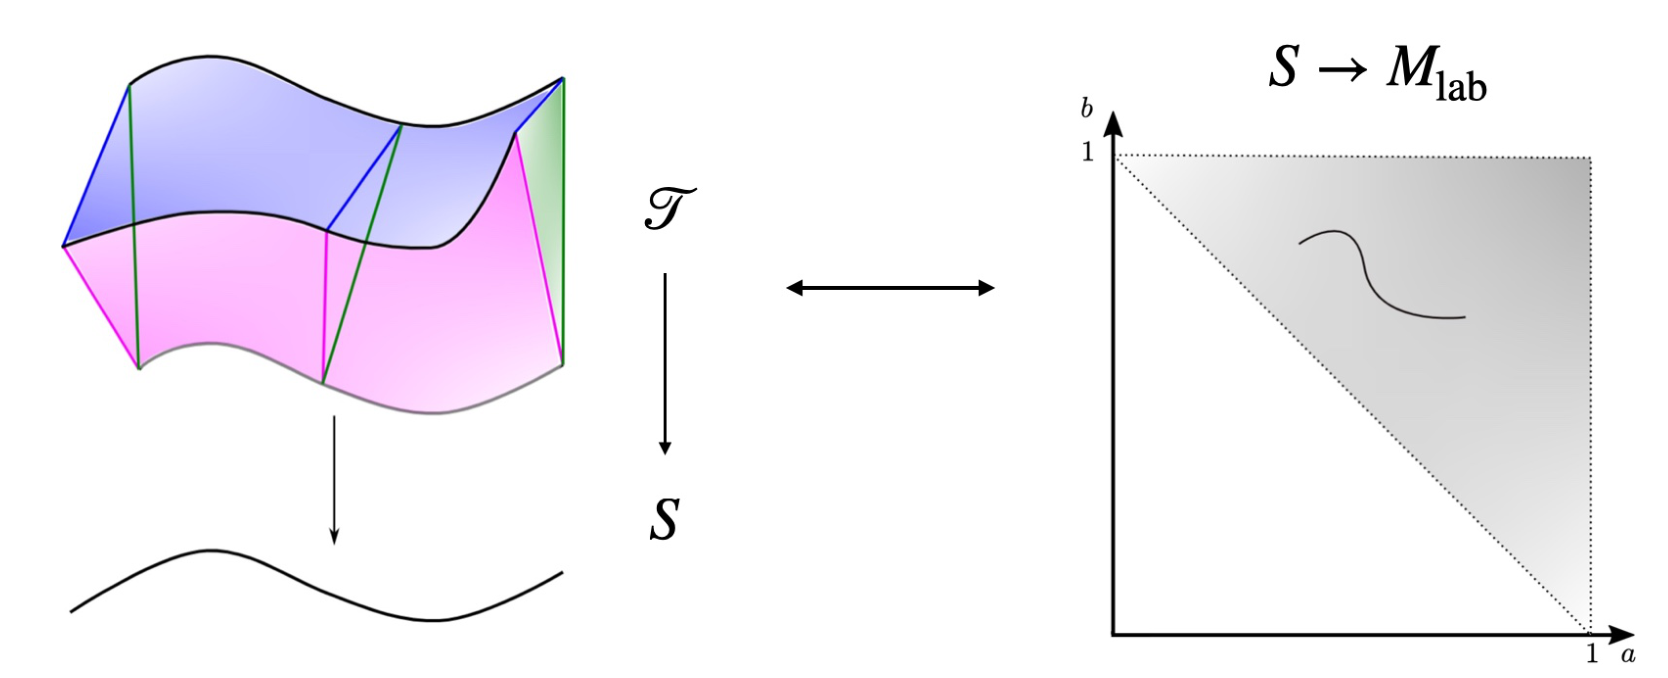
\includegraphics[width=.76\textwidth]{figures/fig-1.3.4.png}
\caption{曲线上的带标号三角形族对应于模空间中的一条弧.}\label{src:1.3.4}
\end{figure}
我们定义带标号三角形的模函子为
\[
\begin{aligned}
F_{M^{\mathrm{lab}}}:&\ \mathsf{Top}\longrightarrow\Sets,\\
&S\longmapsto\{S\text{ 上的带标号三角形族 }(\mathcal T\to S,\sigma_i)\}/(\text{相似}).
\end{aligned}
\]
回忆~\eqref{src:1.2.10}, 将三角形送到其边长的对应, 给出 $F_{M^{\mathrm{lab}}}$ 与下列集合之间的双射: 
\[
M^{\mathrm{lab}}=
\left\{(a,b,c)\ \middle|\
\begin{aligned}
a+b+c&=2\\
0<a&<b+c\\
0<b&<a+c\\
0<c&<a+b
\end{aligned}\right\}.
\]
由于这对每个拓扑空间 $S$ 都延拓为彼此相容的同构
$F_{M^{\mathrm{lab}}}(S)\to\operatorname{Mor}(S,M^{\mathrm{lab}})$, 拓扑空间 $M^{\mathrm{lab}}$ 表出函子 $F_{M^{\mathrm{lab}}}$. 因而存在万有族 $\mathcal T_{\mathrm{univ}}\to M^{\mathrm{lab}}$, 以及截面 $\sigma_i:M^{\mathrm{lab}}\to\mathcal T_{\mathrm{univ}}$.
\begin{figure}[htbp]
\centering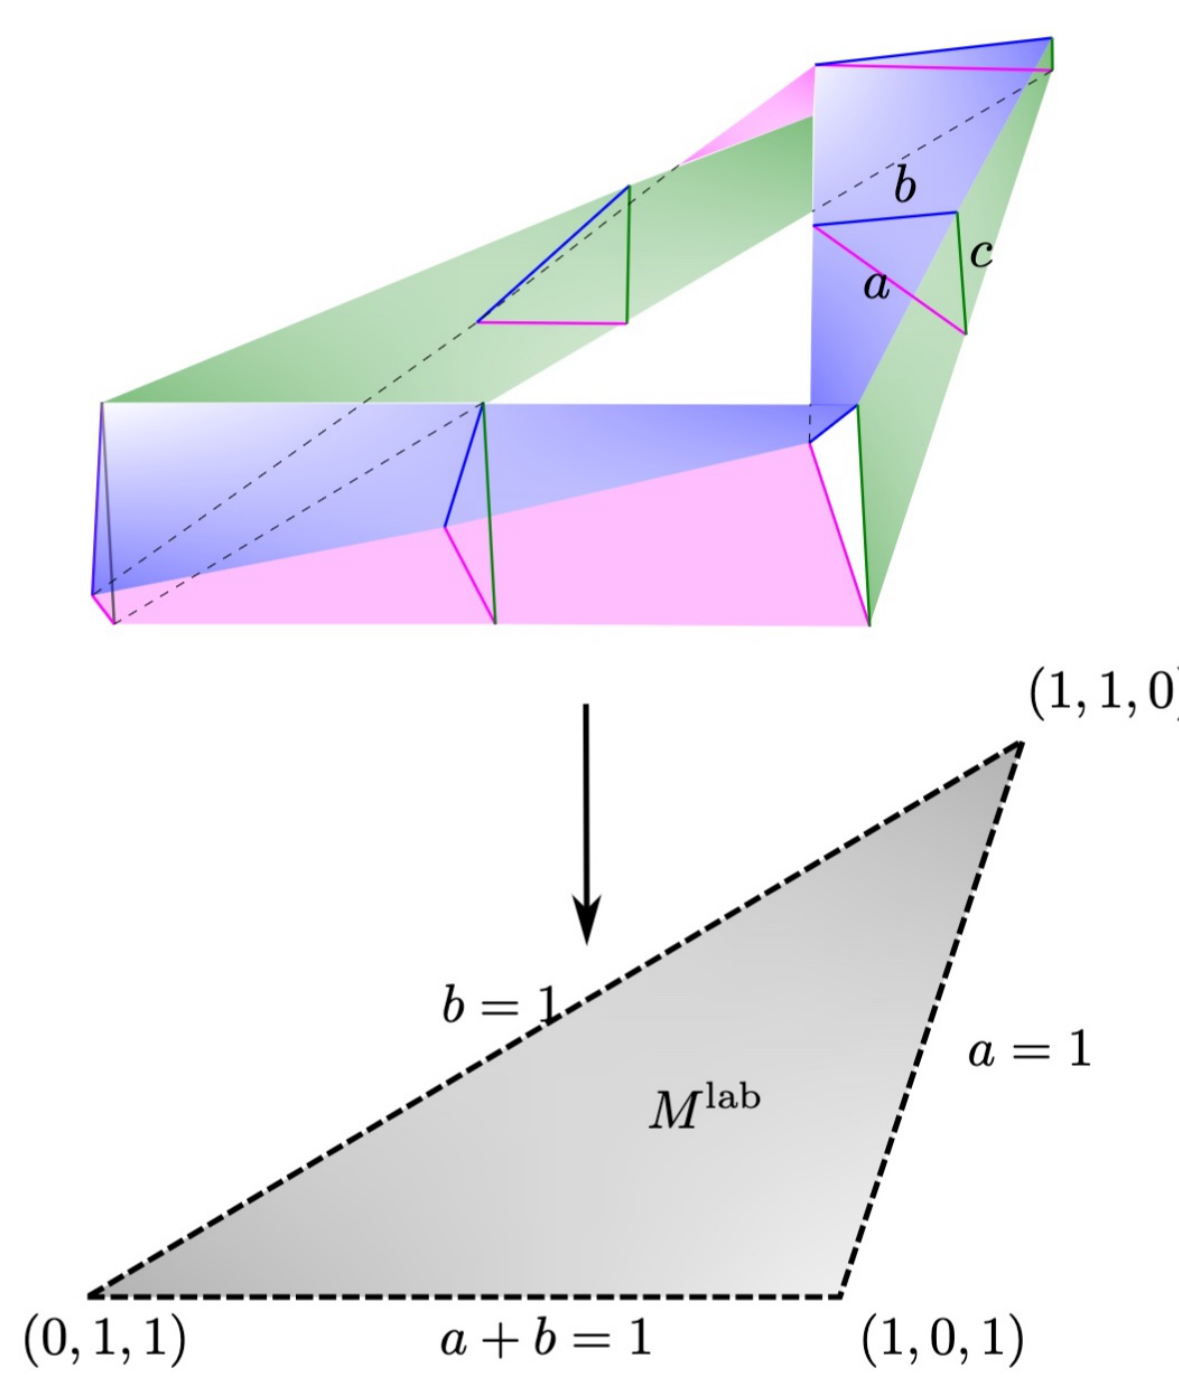
\includegraphics[width=.52\textwidth]{figures/fig-1.3.5.png}
\caption{相似关系下带标号三角形的万有族 $U^{\mathrm{lab}}\to M^{\mathrm{lab}}$.}\label{src:1.3.5}
\end{figure}

\begin{example}[无标号三角形的族]\label{src:1.3.6}
回到例~\bookref{1.2.12}, 我们将\textit{无标号三角形的族}定义为一个纤维丛 $\mathcal T\to S$, 配备连续距离函数 $d:\mathcal T\times_S\mathcal T\to\mathbb R_{\geq0}$, 其在每个纤维上的限制都是度量, 且每个纤维都等距于一个三角形. 两个族 $\mathcal T\to S$ 和 $\mathcal T'\to S$ \textit{相似}, 是指存在 $S$ 上与截面相容的同胚 $f:\mathcal T\to\mathcal T'$, 在各纤维上诱导三角形的相似变换.

我们定义函子
\[
\begin{aligned}
F_{M^{\mathrm{unl}}}:&\ \mathsf{Top}\longrightarrow\Sets,\\
&S\longmapsto\{S\text{ 上的无标号三角形族}\}/(\text{相似}),
\end{aligned}
\]
但已经可以看出, 对象的对称性带来了复杂情况: 每个等边三角形的对称群为 $S_3$, 等腰三角形的对称群则为 $\mathbb Z/2$. 根据命题~\bookref{1.3.30}, 这个函子不可表, 因为存在三角形的非平凡族 $\mathcal T$, 其所有纤维都是相似的三角形. 例如, 利用等边三角形的一个对称变换粘合两个平凡族, 可以构造 $S^1$ 上的一个非平凡三角形族.
\end{example}
\begin{figure}[htbp]
\centering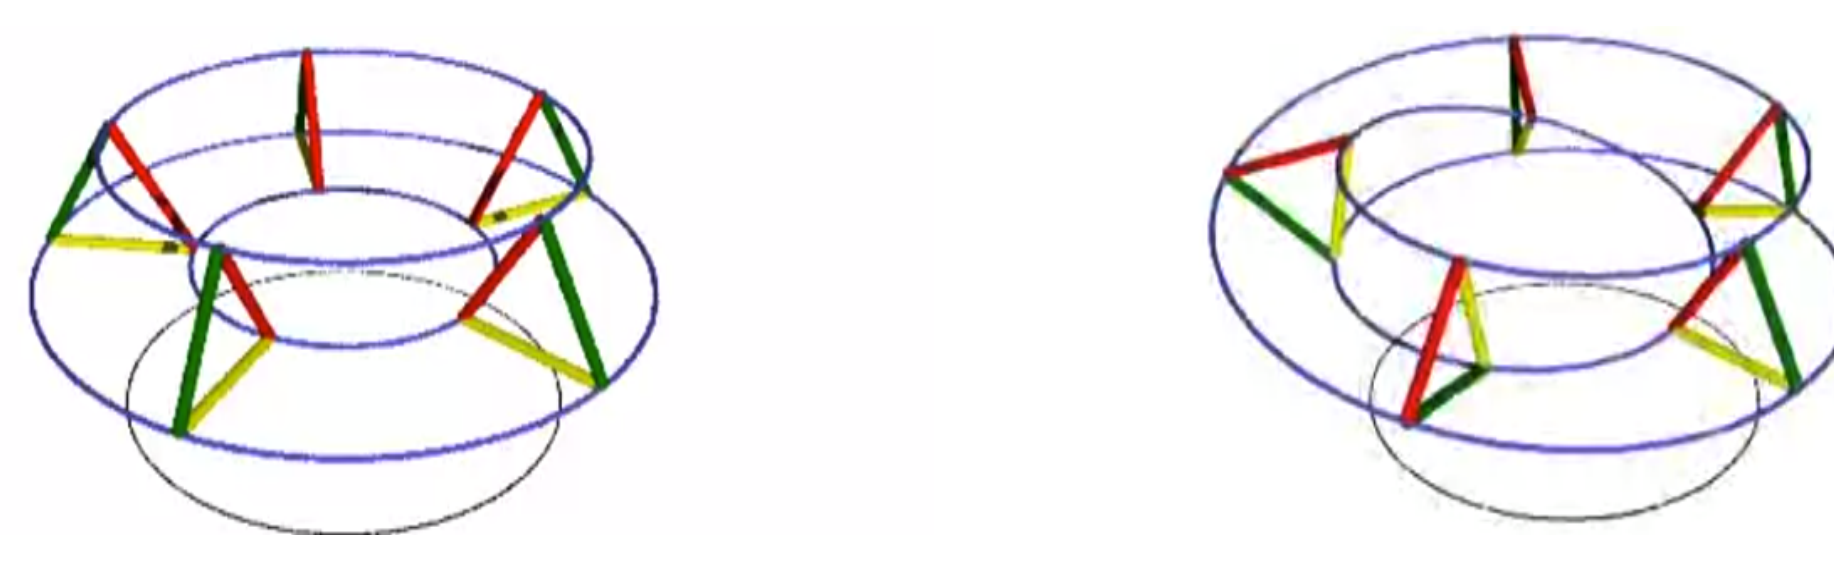
\includegraphics[width=.8\textwidth]{figures/fig-1.3.7.png}
\caption{等边三角形的平凡族(左)与非平凡族(右). 图像取自 Jonathan Wise 制作的视频, 见 \url{http://math.colorado.edu/~jonathan.wise/visual/moduli/index.html}.}\label{src:1.3.7}
\end{figure}

\subsection{曲线, 向量丛与轨道的模函子}\label{src:1.3.2-subsection}
在 $\mathbb C$-概形范畴中定义一个模函子 $F:\Sch/\mathbb C\to\Sets$, 意味着要对每个 $\mathbb C$-概形 $S$, 指定一个由 $S$ 上的对象族组成的集合 $F(S)$; 并对每个 $\mathbb C$-概形态射 $S'\to S$, 指定拉回映射 $F(S)\to F(S')$, 且这些拉回映射与复合相容.

为了获得关于模函子的直观认识, 代入特殊的测试概形总是有益的. 例如, 代入 $S=\operatorname{Spec}\mathbb C$, 就得到由对象组成的底层模集合 $F(\operatorname{Spec}\mathbb C)$. 代入 $S=\mathbb C[\epsilon]/(\epsilon^2)$, 就得到一个二元组的集合, 每个二元组由一个 $\mathbb C$-点和一个切向量组成; 代入一条曲线(或一个离散赋值环), 则得到该曲线上的对象族.

\begin{example}[光滑曲线的模函子]\label{src:1.3.8}
\textit{亏格为 $g$ 的光滑曲线族}是一个光滑, 固有的概形态射 $\mathcal C\to S$, 使得对每个 $s\in S$, 纤维 $\mathcal C_s$ 都是亏格为 $g$ 的连通(光滑固有)曲线.

亏格为 $g$ 的光滑曲线的模函子为
\[
\begin{aligned}
F_{M_g}:&\ \Sch/\mathbb C\longrightarrow\Sets,\\
&S\longmapsto\{\text{亏格为 }g\text{ 的光滑曲线族 }\mathcal C\to S\}/\sim,
\end{aligned}
\]
其中, 两个族 $\mathcal C\to S$ 和 $\mathcal C'\to S$ 等价, 是指存在 $S$ 上的同构 $\mathcal C\to\mathcal C'$. 如果 $S'\to S$ 是一个 $\mathbb C$-概形映射, $\mathcal C\to S$ 是曲线族, 则拉回定义为族 $\mathcal C\times_S S'\to S'$.
\end{example}
\begin{figure}[htbp]
\centering
\begin{tikzpicture}
\node[anchor=south west,inner sep=0] (art) at (0,0) {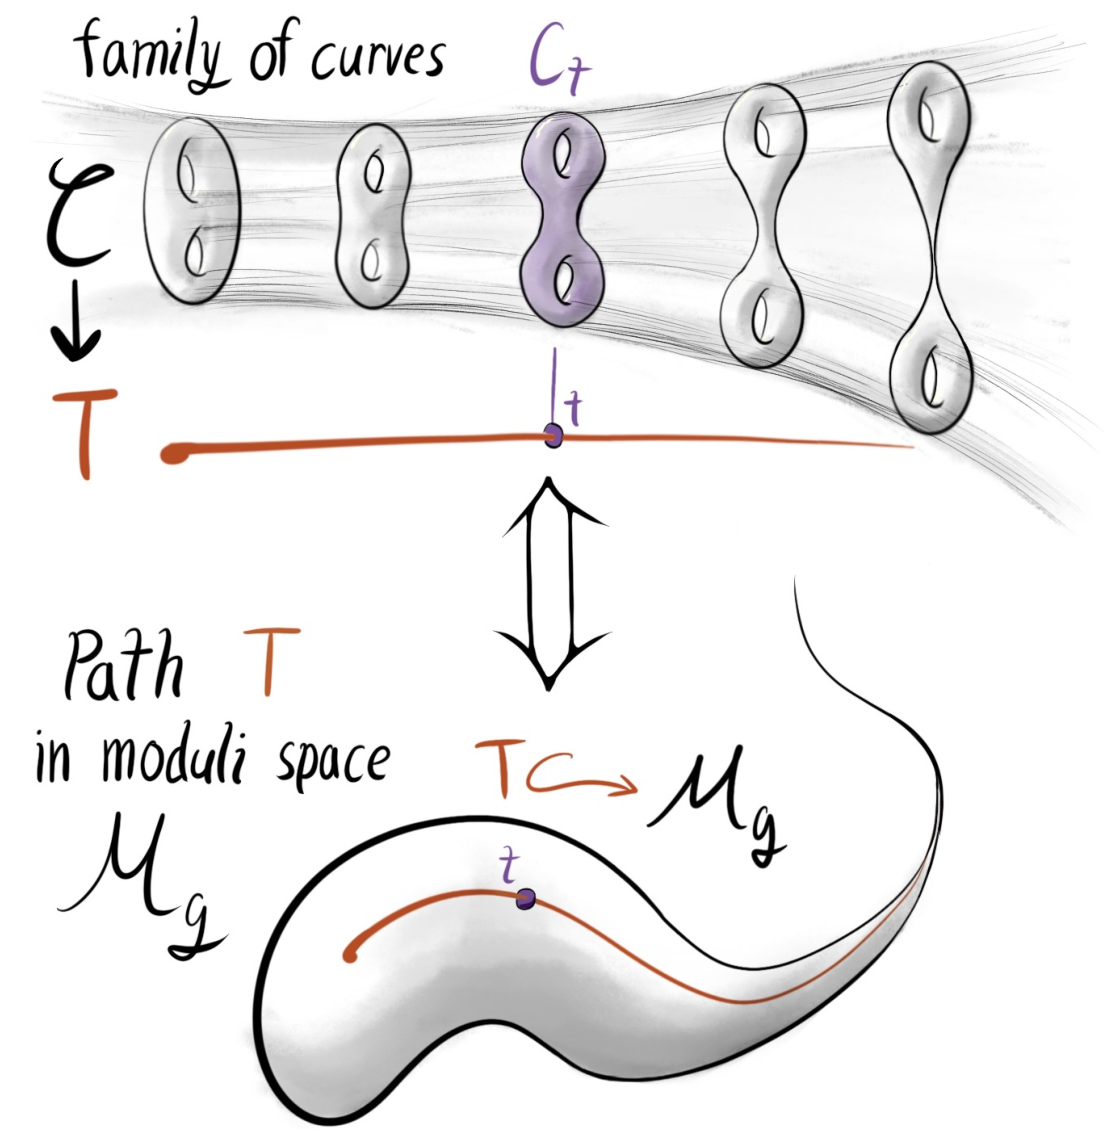
\includegraphics[width=.5\textwidth]{figures/fig-1.3.9.png}};
\begin{scope}[x={(art.south east)},y={(art.north west)}]
\fill[white] (.02,.905) rectangle (.42,1);
\node[font=\small] at (.22,.952) {曲线族};
\fill[white] (.02,.29) rectangle (.38,.47);
\node[font=\small,align=center] at (.20,.38) {模空间\\中的路径};
\end{scope}
\end{tikzpicture}
\caption{曲线族(图中画为 Riemann 曲面)与模空间中的路径之间的对应. 图中还展示了光滑曲线的模空间 $M_g$ 不是紧的: 当路径趋近模空间的边界时, 曲线退化为一条奇异的结点曲线. 后面将看到, 稳定曲线的模空间 $\overline M_g$ 是紧的(定理~\bookref{6.5.23}).}\label{src:1.3.9}
\end{figure}

\begin{example}[曲线上向量丛的模函子]\label{src:1.3.10}
令 $C$ 为 $\mathbb C$ 上一条固定的光滑, 连通射影曲线. $\mathbb C$-概形 $S$ 上的\textit{秩为 $r$, 次数为 $d$ 的向量丛族}, 是 $C\times S$ 上的一个向量丛 $\mathcal E$, 使对每个 $s\in S$, $\mathcal E$ 在 $C_{\kappa(s)}:=C\times_{\mathbb C}\kappa(s)$ 上的限制 $\mathcal E_s:=\mathcal E|_{C_{\kappa(s)}}$ 的秩为 $r$, 次数为 $d$. $C$ 上秩为 $r$, 次数为 $d$ 的向量丛的模函子为
\[
\Sch/\mathbb C\longrightarrow\Sets,\qquad
S\longmapsto
\left\{\begin{gathered}
C\times S\text{ 上的向量丛 }\mathcal E\\
\text{其秩为 }r\text{, 次数为 }d
\end{gathered}\right\}/(\text{同构}).
\]
如果 $f:S'\to S$ 是一个 $\mathbb C$-概形映射, $\mathcal E$ 是 $C\times S$ 上的向量丛, 则拉回定义为 $C\times S'$ 上的向量丛 $(\mathrm{id}\times f)^*\mathcal E$.
\end{example}
我们将在第~\bookref{1.3.5-subsection}~小节看到, 这两个函子都不可表, 相应地, 也都不存在细模空间.

\begin{example}[轨道的模函子]\label{src:1.3.11}
考虑 $\mathbb C$ 上的代数群 $G$ 在 $\mathbb C$-概形 $X$ 上的作用. 对每个 $\mathbb C$-概形 $S$, 抽象群 $G(S)$ 在集合 $X(S)$ 上作用; 事实上, 给出这样的作用, 并使其关于 $S$ 具有函子性, 就唯一确定了该群作用(习题~\bookref{B.1.11}). 我们可以考虑函子
\[
\Sch/\mathbb C\longrightarrow\Sets,\qquad S\longmapsto X(S)/G(S).
\]
这是商的模函子的一个十分朴素的候选, 即使对自由作用, 也远远不能做到可表(见习题~\bookref{1.3.38}). 我们将在 \S\bookref{1.6.5-subsection} 中修改这个例子.
\end{example}
某些情况下, 你可能确切知道要参数化哪些对象, 但引入族的概念未必容易. 对对象族也可能有几个候选概念, 它们可能在同一个拓扑空间上给出不同的概形结构. 高维簇的模就是这样的例子(见 \S\bookref{10.1.3-subsection}).

\subsection{Yoneda 引理与可表函子}\label{src:1.3.3-subsection}
\begin{epigraph}
Yoneda 引理是数学中最难的平凡事实.
\epigraphauthor{Dan Piponi}
\end{epigraph}
遵循 Grothendieck 的思想, 我们将通过研究到概形 $X$ 的所有映射来研究 $X$!这个思维上的技巧正是函子方法的核心: 一个几何对象由它与所有其他对象之间的关系所决定. Yoneda 引理将此严格化: 对范畴 $\mathcal C$ 的一个对象 $X$, 反变函子
\[
h_X:\mathcal C\longrightarrow\Sets,\qquad S\longmapsto\operatorname{Mor}(S,X)
\]
恢复对象 $X$ 本身.

\begin{lemma}[Yoneda 引理]\label{src:1.3.12}
令 $\mathcal C$ 为一个范畴, $X$ 为其中一个对象. 对每个反变函子 $G:\mathcal C\to\Sets$, 映射
\[
\operatorname{Mor}(h_X,G)\longrightarrow G(X),\qquad
\alpha\longmapsto\alpha_X(\mathrm{id}_X)
\]
为双射, 且关于 $X$ 和 $G$ 都具有函子性. 这里, 左边表示自然变换 $h_X\to G$ 的集合, $\alpha_X$ 表示映射 $h_X(X)=\operatorname{Mor}(X,X)\to G(X)$.
\end{lemma}
\begin{exercise}[一生中至少应做一次]\label{src:1.3.13}
证明 Yoneda 引理. 为此, 必须准确说明``关于 $X$ 和 $G$ 都具有函子性''的含义.
\end{exercise}
\begin{caution}\label{src:1.3.14}
全书中, 我们将一贯滥用记号, 不区分元素 $g\in G(X)$ 与对应的态射 $h_X\to G$; 后者又常简写为 $X\to G$.
\end{caution}
\begin{definition}[可表函子与细模空间]\label{src:1.3.15}
称函子 $F:\Sch\to\Sets$ \newterm{可由概形表出}{representable by a scheme}, 是指存在概形 $X$ 和函子同构 $F\xrightarrow{\sim}h_X$.

当 $F$ 为模函子, 且可由概形 $M$ 表出时, 称 $M$ 为\newterm{细模空间}{fine moduli space}.
\end{definition}
由 Yoneda 引理(\bookref{1.3.12}), 如果一个函子可表, 那么它可由唯一的概形表出. 我们的一个目标, 就是理解给定的模函子 $F$ 何时具有细模空间, 即何时可由概形表出.

\begin{example}[射影空间作为函子]\label{src:1.3.16}
由~\cite[定理 II.7.1]{Har77}, 存在具有函子性的双射
\[
\operatorname{Mor}(S,\mathbb P^n_{\mathbb Z})\cong
\left\{(L,s_0,\ldots,s_n)\ \middle|\
\begin{gathered}
L\text{ 是 }S\text{ 上的线丛, 由截面}\\
s_0,\ldots,s_n\in\Gamma(S,L)\text{ 整体生成}
\end{gathered}\right\}/\sim,
\]
其中, $(L,s_i)\sim(L',s'_i)$ 是指存在同构 $\alpha:L\to L'$, 使对所有 $i$ 都有 $s_i=\alpha^*s'_i$. 换言之, 右边的函子可由概形 $\mathbb P^n_{\mathbb Z}$ 表出. 截面 $s_i$ 整体生成这一条件, 意味着对每个 $x\in S$, 至少有一个截面 $s_i(x)\in L\otimes\kappa(x)$ 非零; 等价地, $(s_0,\ldots,s_n):\mathcal O_S^{\oplus n+1}\to L$ 为满射.
\end{example}

\begin{example}[Grassmann 函子]\label{src:1.3.17}
作为集合, Grassmann 簇 $\operatorname{Gr}(q,n)$ 参数化 $n$ 维空间的 $q$ 维商.\footnote{也可以将这些点视为 $q$ 维子空间, 但在本讲义中, 我们遵循 Grothendieck 使用商的约定.} 然而, 概形 $S$ 上的 $q$ 维商的族是什么?一个朴素的猜测可能是商 $p:\mathcal O_S^n\twoheadrightarrow\mathcal O_S^k$, 但这根本不可能可表(见习题~\bookref{1.3.38}). 射影空间的情形提示我们将 \newterm{Grassmann 函子}{Grassmannian functor}定义为
\[
\begin{aligned}
\operatorname{Gr}(q,n):&\ \Sch\longrightarrow\Sets,\\
&S\longmapsto
\left\{[\mathcal O_S^{\oplus n}\twoheadrightarrow Q]\ \middle|\ Q\text{ 为秩 }q\text{ 的向量丛}\right\}/\sim,
\end{aligned}
\]
其中, $[p:\mathcal O_S^{\oplus n}\twoheadrightarrow Q]\sim[p':\mathcal O_S^{\oplus n}\twoheadrightarrow Q']$, 是指存在同构 $\Psi:Q\xrightarrow{\sim}Q'$ 使图
\[
\begin{tikzcd}
\mathcal O_S^{\oplus n}\arrow[r,"p"]\arrow[dr,"p'"'] & Q\arrow[d,"\Psi","\sim"']\\
&Q'
\end{tikzcd}
\]
交换(即 $p'=\Psi\circ p$); 等价地, $\ker(p)=\ker(p')$. 拉回以自然方式定义.

后面我们将证明, $\operatorname{Gr}(q,n)$ 可由一个在 $\mathbb Z$ 上射影的概形表出(定理~\bookref{2.1.1}). 这一结果的证明很好地说明了函子方法的用处, 也是 Hilb 和 Quot 可表性(定理~\bookref{2.1.2}~和~\bookref{2.1.3})的热身.
\end{example}
以下习题将帮助你练习函子方法.

\begin{exercise}[仿射空间与射影空间]\label{src:1.3.18}
令 $S$ 为概形, $E$ 为 $S$ 上的向量丛.
\begin{enumerate}[(a)]
\item 证明仿射空间 $\mathbb A(E):=\mathcal{S}pec_S(\operatorname{Sym}^*E)$ 表出将 $f:T\to S$ 送到 $\Gamma(T,f^*E^\vee)$ 的函子, 其中 $E^\vee:=\mathcal{H}om_{\mathcal O_S}(E,\mathcal O_S)$. 注意, $\mathbb A(E)$ 的一个 $\Bbbk$-点是 $E\otimes_{\mathcal O_S}\Bbbk$ 的对偶中的一个元素.\footnote{这与~\cite[习题 5.18, 162 页的定义]{Har77}, \cite[II.4.1.1]{EGA}~以及~\cite[Tag 01OB]{SP}~一致; 但须注意, 有些作者在定义 $\mathbb A(E)$ 和 $\mathbb P(E)$ 时, 使用对偶 $E^\vee$ 而非 $E$.} 还应注意特殊情形 $\mathbb A(\mathcal O_S^{\oplus n})\cong\mathbb A_S^n$.
\item 证明 $E$ 的射影化 $\mathbb P(E):=\mathcal{P}roj_S(\operatorname{Sym}^*E)$ 表出函子
\[
\begin{aligned}
\Sch/S&\longrightarrow\Sets,\\
(T\xrightarrow{f}S)&\longmapsto
\{q:f^*E\twoheadrightarrow L\text{, 其中 }L\text{ 为 }T\text{ 上的线丛}\}/\sim,
\end{aligned}
\]
其中, $[q:f^*E\twoheadrightarrow L]\sim[q':f^*E\twoheadrightarrow L']$ 是指 $\ker(q)=\ker(q')$(等价地, 存在同构 $\alpha:L\to L'$, 使 $q'=\alpha\circ q$). 注意, $E$ 自然等同于 $\mathcal O_{\mathbb P(E)}(1)$ 沿 $\mathbb P(E)\to S$ 的推前; 当 $E$ 平凡时, 有等同 $\mathbb P(\mathcal O_S^{n+1})\cong\mathbb P^n$.
\end{enumerate}
\end{exercise}
\begin{exercise}[简单, 适于练习]\label{src:1.3.19}
给出以下对象的函子描述: 
\begin{enumerate}[(a)]
\item $\mathbb A^n\setminus0$; 
\item $\operatorname{Spec}\Bbbk[x_1,\ldots,x_n]/(f_1,\ldots,f_m)$; 
\item $\mathcal{S}pec_S\mathcal A$, 其中 $\mathcal A$ 是概形 $S$ 上的拟凝聚代数层; 以及
\end{enumerate}
\end{exercise}
\begin{exercise}[困难]\label{src:1.3.20}
若 $S$ 为概形, $\mathcal A$ 为正分次 $\mathcal O_S$-代数, 给出 $\mathcal{P}roj_S\mathcal A$ 的函子描述.(另见~\cite[Tag 01NS]{SP}.)
\end{exercise}
\begin{exercise}[中等, 适于练习]\label{src:1.3.21}
令 $X$ 为概形, $F_1$ 和 $F_2$ 为 $X$ 上的向量丛. 证明函子
\[
\begin{aligned}
\underline{\mathcal{H}om}_{\mathcal O_X}(F_1,F_2):&\ \Sch/X\longrightarrow\Sets,\\
&(f:T\to X)\longmapsto\operatorname{Hom}_{\mathcal O_T}(f^*F_1,f^*F_2)
\end{aligned}
\]
可由 $\mathbb A(\mathcal{H}om_{\mathcal O_X}(F_1,F_2)^\vee)\to X$ 表出.

注意以下记号的区别: 
\begin{itemize}
\item $\operatorname{Hom}_{\mathcal O_X}(F_1,F_2)$: $\mathcal O_X$-模同态群; 
\item $\mathcal{H}om_{\mathcal O_X}(F_1,F_2)$: $\mathcal O_X$-模同态层; 
\item $\underline{\mathcal{H}om}_{\mathcal O_X}(F_1,F_2)$: 参数化 $\mathcal O_X$-模同态的函子或概形.
\end{itemize}
\end{exercise}
\begin{exercise}[中等]\label{src:1.3.22}
令 $X$ 为域 $\Bbbk$ 上的概形, $F_1$ 和 $F_2$ 为 $X$ 上的向量丛. 证明从仿射 $\Bbbk$-概形范畴出发的函子
\[
\begin{aligned}
\underline{\operatorname{Ext}}^1_{\mathcal O_X}(F_1,F_2):&\
\mathsf{AffSch}/\Bbbk\longrightarrow\Sets,\\
&T\longmapsto\operatorname{Ext}^1_{\mathcal O_{X\times T}}(p_1^*F_1,p_1^*F_2)
\end{aligned}
\]
可由 $\mathbb A(\operatorname{Ext}^1_{\mathcal O_X}(F_1,F_2)^\vee)$ 表出. 另见~\cite[\S7.3]{LP97}~和命题~\bookref{9.2.13}.
\end{exercise}
\begin{exercise}[中等]\label{src:1.3.23}
令 $S$ 为 Noether 概形, $E\to F$ 为 $\mathbb P_S^n$ 上的凝聚层同态, 其中 $F$ 在 $S$ 上平坦. 证明由下式定义的 $S$ 的子函子(更准确地说, 是 $h_S=\operatorname{Mor}(-,S)$ 的子函子)
\[
\Sch\longrightarrow\Sets,\qquad
T\longmapsto\{T\to S\text{ 的态射, 使 }E_T\to F_T\text{ 为零}\}
\]
可由 $X$ 的一个闭子概形表出.
\end{exercise}
\begin{exercise}[Weil 限制, 困难]\label{src:1.3.24}
设 $S'\to S$ 为概形态射. 态射 $X'\to S'$ 的 \newterm{Weil 限制}{Weil restriction}是函子
\[
\operatorname{Re}_{S'/S}(X'):\Sch/S\longrightarrow\Sets,\qquad
(T\to S)\longmapsto X'(T\times_S S').
\]
\begin{enumerate}[(1)]
\item 若 $\Bbbk/\Bbbk'$ 为次数 $d$ 的域扩张, 证明 $\operatorname{Re}_{\Bbbk'/\Bbbk}\mathbb A^1\cong\mathbb A^d$.
\item 证明 $T:=\operatorname{Re}_{\mathbb C/\mathbb R}(\mathbb G_{m,\mathbb C})$ 为 $\mathbb R$ 上的代数群, 它是秩为 $2$ 的非分裂环面, 即 $T\times_{\mathbb R}\mathbb C\cong\mathbb G_{m,\mathbb C}^2$, 但 $T\not\cong\mathbb G_{m,\mathbb R}^2$.
\item (困难)假设 $S'\to S$ 有限且平坦, 并且对每个 $s\in S$, 纤维 $X'_s$ 中的任意有限点集都包含于一个仿射开集内, 则 $\operatorname{Re}_{S'/S}(X')$ 可表. 另见~\cite[定理 $7.4$]{BLR90}.
\end{enumerate}
\end{exercise}

\subsection{万有族}\label{src:1.3.4-subsection}
\begin{definition}\label{src:1.3.25}
若 $F:\Sch\to\Sets$ 为模函子, 且通过函子同构 $\alpha:F\xrightarrow{\sim}h_M$ 可由概形 $M$ 表出, 则 $F$ 的\textit{万有族}是对象 $u\in F(M)$, 它在 $\alpha$ 下对应于恒等态射 $\mathrm{id}_M\in h_M(M)=\operatorname{Mor}(M,M)$.
\end{definition}
\begin{exercise}[简单但重要]\label{src:1.3.26}
令 $F:\Sch\to\Sets$ 为可由概形 $M$ 表出的函子, $u\in F(M)$ 为万有族. 若 $a\in F(T)$ 为概形 $T$ 上的一个对象, 对应于映射 $f_a:T\to M$, 证明对象 $a$ 为 $u$ 沿 $f_a$ 的拉回, 即 $a=F(f_a)(u)$.
\end{exercise}
暂且放下疑虑, 假设确实存在一个概形 $M_g$, 表出亏格为 $g$ 的光滑曲线的模函子(例~\bookref{1.3.8}). 那么恒等映射 $M_g\to M_g$ 就对应于一个亏格为 $g$ 的曲线族 $U_g\to M_g$, 满足以下万有性质: 对概形 $S$ 上的每个光滑曲线族 $\mathcal C\to S$, 存在唯一映射 $S\to M_g$ 和 Cartesian 图
\[
\begin{tikzcd}
\mathcal C\arrow[r]\arrow[d]\arrow[dr,phantom,"\square"] & U_g\arrow[d]\\
S\arrow[r] & M_g.
\end{tikzcd}
\]
映射 $S\to M_g$ 将点 $s\in S$ 送到曲线 $[\mathcal C_s]\in M_g$. 虽然不存在表出这个模函子的概形 $M_g$, 却存在参数化光滑曲线的代数叠 $\mathcal M_g$, 并配备万有族; 见 \S\bookref{4.1.31}.
\begin{figure}[htbp]
\centering
\begin{tikzpicture}
\node[anchor=south west,inner sep=0] (art) at (0,0) {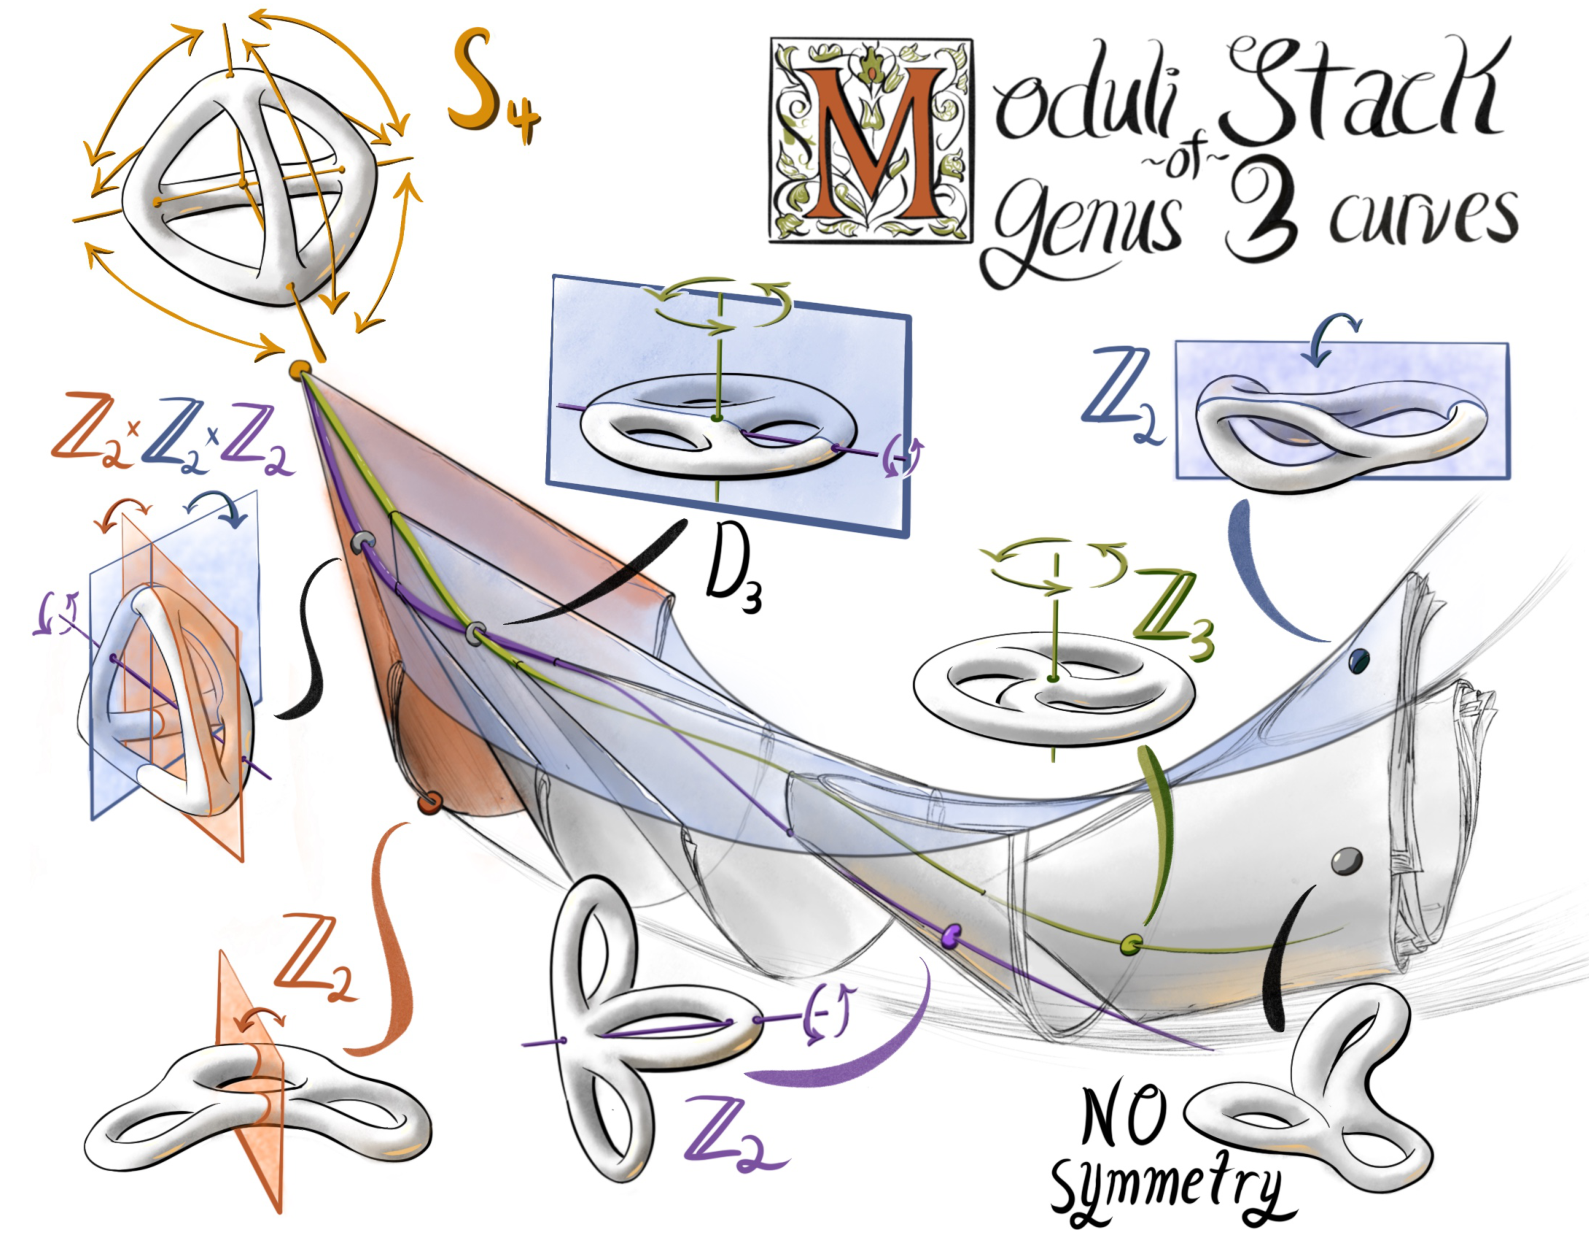
\includegraphics[width=.72\textwidth]{figures/fig-1.3.27.png}};
\begin{scope}[x={(art.south east)},y={(art.north west)}]
\fill[white] (.47,.755) rectangle (1,1);
\node[font=\small,align=center] at (.735,.89) {亏格为 $3$ 的曲线的模叠};
\fill[white] (.676,.085) rectangle (.739,.151);
\fill[white] (.655,.015) rectangle (.817,.079);
\node[font=\scriptsize] at (.73,.045) {无对称性};
\end{scope}
\end{tikzpicture}
\caption{$\mathcal M_3$ 的万有族示意图, 着重描绘具有非平凡对称群的 Riemann 曲面.}\label{src:1.3.27}
\end{figure}
\begin{example}\label{src:1.3.28}
射影空间的模函子 (例~\bookref{1.3.16}) 的万有族, 是 $\mathbb P^n$ 上的线丛 $\mathcal O(1)$, 连同截面
\[
x_0,\ldots,x_n\in\Gamma(\mathbb P^n,\mathcal O(1)).
\]
\end{example}
\begin{example}[代数拓扑中的分类空间]\label{src:1.3.29}
令 $G$ 为拓扑群, $\mathsf{Top}^{\mathrm{para}}$ 为仿紧拓扑空间组成的范畴, 其中态射定义到同伦等价. 代数拓扑中的一个定理断言, 函子
\[
\mathsf{Top}^{\mathrm{para}}\longrightarrow\Sets,\qquad
S\longmapsto\{\text{主 }G\text{-丛 }P\to S\}/(\text{同构})
\]
可由一个拓扑空间表出, 我们将它记作 $BG$, 并称为\newterm{分类空间}{classifying space}. 万有族通常记作 $EG\to BG$. 例如, 分类空间 $B\mathbb C^*$ 是无穷维流形 $\mathbb{CP}^{\infty}$. 然而, 在代数几何中, \newterm{分类叠}{classifying stack} $B\mathbb G_{m,\mathbb C}$ 是维数为 $-1$ 的代数叠.
\end{example}

\subsection{不可表模函子的例子}\label{src:1.3.5-subsection}
若 $F:\Sch/\mathbb C\to\Sets$ 为模函子, 那么具有非平凡自同构的对象 $E\in F(\mathbb C)$ 可能阻止函子 $F$ 的可表性. 原因是, 我们可以利用这个自同构粘合平凡族, 构造概形 $S$ 上的非平凡族 $\mathcal E$, 使每个纤维 $\mathcal E_s$(即 $\mathcal E$ 沿 $\operatorname{Spec}\mathbb C\to S$ 的拉回)都同构于 $E$.
\begin{proposition}\label{src:1.3.30}
令 $F:\Sch/\mathbb C\to\Sets$ 为模函子. 如果存在簇 $S$ 上的对象族 $\mathcal E\in F(S)$, 满足
\begin{enumerate}[(a)]
\item 对 $s\in S(\mathbb C)$, 纤维 $\mathcal E_s$ 彼此同构; 以及
\item 族 $\mathcal E$ 非平凡, 即它不等于任何对象 $E\in F(\mathbb C)$ 沿结构映射 $S\to\operatorname{Spec}\mathbb C$ 的拉回, 
\end{enumerate}
那么 $F$ 不可表.
\end{proposition}
\begin{proof}
反设 $F$ 可由概形 $X$ 表出. 由条件 (a), 限制 $E:=\mathcal E_s$ 与 $s\in S(\mathbb C)$ 无关, 并确定唯一的点 $x\in X(\mathbb C)$. 由于 $S$ 约化, 映射 $S\to X$ 分解为 $S\to\operatorname{Spec}\mathbb C\xrightarrow{x}X$. 这意味着族 $\mathcal E$ 为沿常值映射 $S\to\operatorname{Spec}\mathbb C\xrightarrow{x}X$ 的拉回, 即 $\mathcal E$ 为平凡族, 与条件 (b) 矛盾.
\end{proof}
\begin{exercise}[简单]\label{src:1.3.31}
证明将概形 $S$ 送到 $S$ 上的向量丛同构类的集合的模函子 $F:\Sch/\mathbb C\to\Sets$ 不可表.
\end{exercise}
\begin{example}[椭圆曲线的模]\label{src:1.3.32}
一条\textit{椭圆曲线}是一个二元组 $(E,p)$, 其中 $E$ 为亏格 $1$ 的光滑, 连通射影曲线, $p\in E(\mathbb C)$. 概形 $S$ 上的\textit{椭圆曲线族}是一个二元组 $(\mathcal E\to S,\sigma)$, 其中 $\mathcal E\to S$ 是带有截面 $\sigma:S\to\mathcal E$ 的光滑固有态射, 使对每个 $s\in S$, 纤维 $(\mathcal E_s,\sigma(s))$ 为剩余域 $\kappa(s)$ 上的椭圆曲线. 椭圆曲线的模函子为
\[
\begin{aligned}
F_{M_{1,1}}:&\ \Sch\longrightarrow\Sets,\\
&S\longmapsto\{\text{椭圆曲线族 }(\mathcal E\to S,\sigma)\}/\sim,
\end{aligned}
\]
其中, $(\mathcal E\to S,\sigma)\sim(\mathcal E'\to S,\sigma')$ 是指存在与截面相容的 $S$-同构 $\alpha:\mathcal E\to\mathcal E'$(即 $\sigma'=\alpha\circ\sigma$).
\end{example}
\begin{exercise}[适于练习]\label{src:1.3.33}
考虑在 $\mathbb A^1\setminus0$(坐标为 $t$)上由下图定义的椭圆曲线族: 
\[
\begin{tikzcd}[column sep=large]
\mathcal E:=V(y^2z-x^3+tz^3)\arrow[r,hook]\arrow[d] &
(\mathbb A^1\setminus0)\times\mathbb P^2\\
\mathbb A^1\setminus0 &
\end{tikzcd}
\]
截面 $\sigma:\mathbb A^1\setminus0\to\mathcal E$ 由 $t\mapsto[0,1,0]$ 给出. 证明 $(\mathcal E\to\mathbb A^1\setminus0,\sigma)$ 满足命题~\bookref{1.3.30}~中的 (a) 和 (b), 并推得 $F_{M_{1,1}}$ 不可表.
\end{exercise}
\begin{example}[光滑曲线的模函子]\label{src:1.3.34}
令 $C$ 为一条具有非平凡自同构 $\alpha\in\operatorname{Aut}(C)$ 的曲线, $N$ 为结点三次曲线, 可以将其理解为把 $\mathbb P^1$ 上的点 $0$ 和 $\infty$ 粘合而成的曲线. 取平凡族 $\pi:C\times\mathbb P^1\to\mathbb P^1$, 通过自同构 $\alpha$ 将纤维 $\pi^{-1}(0)$ 与 $\pi^{-1}(\infty)$ 粘合, 就能构造一个族 $\mathcal C\to N$. 要证明光滑曲线的模函子 $\Sch/\mathbb C\to\Sets$ 不可表, 只须证明 $\mathcal C\to N$ 非平凡.
\end{example}
\begin{figure}[htbp]
\centering
\begin{tikzpicture}
\node[anchor=south west,inner sep=0] (art) at (0,0) {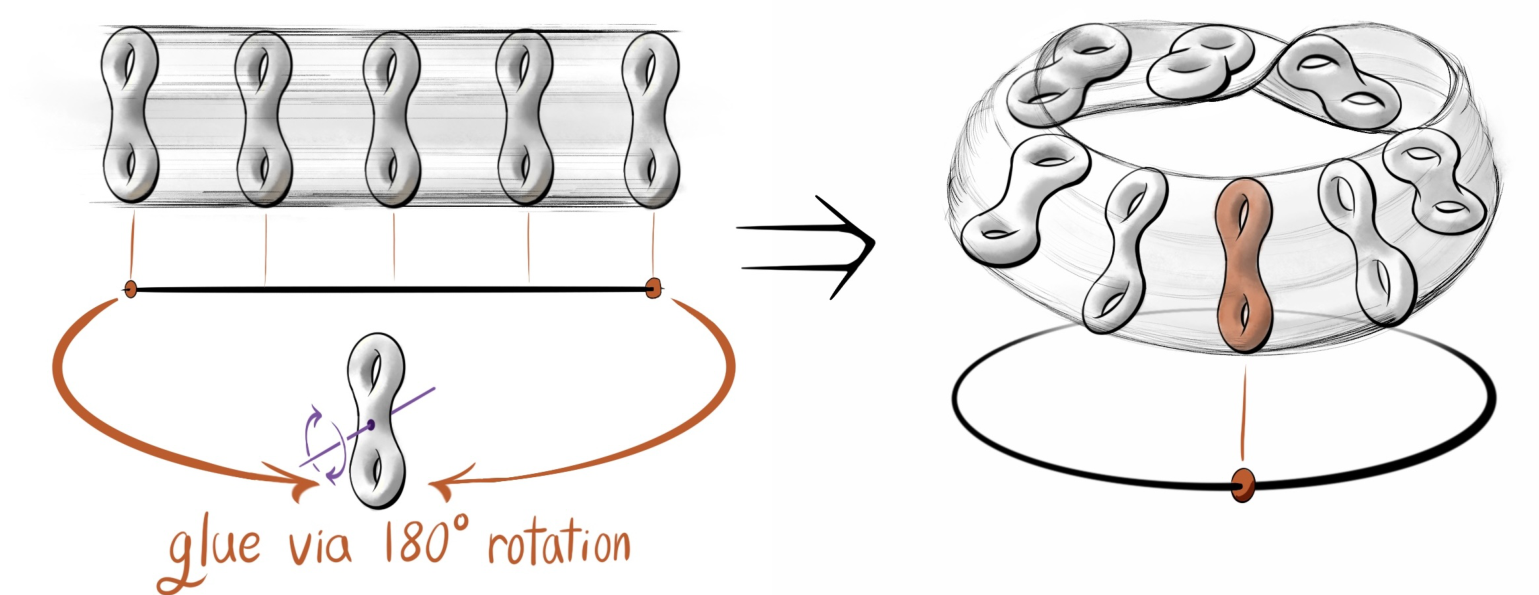
\includegraphics[width=.72\textwidth]{figures/fig-1.3.35.png}};
\begin{scope}[x={(art.south east)},y={(art.north west)}]
\fill[white] (.07,0) rectangle (.44,.15);
\node[font=\scriptsize] at (.26,.06) {通过 $180^\circ$ 旋转粘合};
\end{scope}
\end{tikzpicture}
\caption{通过非平凡自同构粘合平凡族, 得到一个由 Riemann 曲面组成的 Möbius 带.}\label{src:1.3.35}
\end{figure}
\begin{exercise}[补充细节]\label{src:1.3.36}
证明 $\mathcal C\to N$ 为非平凡族.
\end{exercise}
\begin{exercise}[适于练习]\label{src:1.3.37}
证明曲线 $C$ 上的向量丛的模函子不可表.
\end{exercise}

\subsection{概形是大 Zariski 拓扑中的层}\label{src:1.3.6-subsection}
若 $F:\Sch\to\Sets$ 可由概形 $X$ 表出, 则 $F$ 必为\newterm{大 Zariski 拓扑}{big Zariski topology}中的层. 也就是说, 对每个概形 $S$, 在 $S$ 的 Zariski 拓扑上, 将开子集 $U\subseteq S$ 送到集合 $F(U)$ 所定义的预层, 是 $S$ 的 Zariski 拓扑上的层. 这只是对``到固定概形 $X$ 的态射可以唯一粘合''的另一种表述. 因此, 不满足层条件便构成给定模函子 $F$ 可表性的另一种障碍.
\begin{exercise}[适于练习]\label{src:1.3.38}
\begin{enumerate}[(a)]
\item 证明下列朴素的 Grassmann 函子不可表: 
\[
F:\Sch\longrightarrow\Sets,\qquad
S\longmapsto\{q:\mathcal O_S^n\twoheadrightarrow\mathcal O_S^k\text{ 的商}\}/\sim.
\]
\item 在 $\mathbb G_m$ 对 $\mathbb A^{n+1}\setminus0$ 的通常数乘作用下, 证明函子 $S\mapsto(\mathbb A^{n+1}\setminus0)(S)/\mathbb G_m(S)$ 不是层.
\end{enumerate}
\end{exercise}
非平凡自同构的存在, 常常意味着给定的模函子不是大 Zariski 拓扑中的层.
\begin{example}\label{src:1.3.39}
考虑例~\bookref{1.3.8}~中的光滑曲线的模函子 $F_{M_g}$. 令 $\{S_i\}$ 为概形 $S$ 的 Zariski 开覆盖, 假设 $\mathcal C_i\to S_i$ 为光滑曲线族, 并在交集 $S_{ij}:=S_i\cap S_j$ 上有同构 $\alpha_{ij}:\mathcal C_i|_{S_{ij}}\xrightarrow{\sim}\mathcal C_j|_{S_{ij}}$. 要求 $F_{M_g}$ 为层(当限制到 $S$ 的 Zariski 拓扑时), 意味着这些族 $\mathcal C_i\to S_i$ 可以唯一粘合成一个曲线族 $\mathcal C\to S$. 然而, 我们并未要求同构 $\alpha_i$ 在三重交集上相容(即 $\alpha_{ij}|_{S_{ijk}}\circ\alpha_{jk}|_{S_{ijk}}=\alpha_{ik}|_{S_{ijk}}$), 而这却是粘合概形所必需的~\cite[习题 II.2.12]{Har77}. 因此, $F_{M_g}$ 不是层.
\end{example}
\begin{exercise}\label{src:1.3.40}
通过明确给出一个概形 $S$, 一个开覆盖 $\{S_i\}$, 以及无法粘合为 $S$ 上的族的 $S_i$ 上的曲线族, 证明光滑曲线和椭圆曲线的模函子都不是层.
\end{exercise}

\subsection{函子的运用}\label{src:1.3.7-subsection}
反变函子 $F:\Sch\to\Sets$ 组成范畴 $\operatorname{Fun}(\Sch,\Sets)$, 其中态射为自然变换. 这个范畴具有纤维积: 给定态射 $\alpha:F\to G$ 和 $\beta:G'\to G$, 定义
\[
\begin{aligned}
F\times_G G':&\ \Sch\longrightarrow\Sets,\\
&S\longmapsto
\{(a,b)\in F(S)\times G'(S)\mid\alpha_S(a)=\beta_S(b)\in G(S)\}.
\end{aligned}
\]
\begin{exercise}[简单]\label{src:1.3.41}
证明 $F\times_G G'$ 满足 $\operatorname{Fun}(\Sch,\Sets)$ 中纤维积的万有性质.
\end{exercise}
\begin{definition}\label{src:1.3.42}
\begin{enumerate}[(1)]
\item 称反变函子之间的态射 $F\to G$ \newterm{可由概形表出}{representable by schemes}, 是指对来自概形 $S$ 的每个映射 $S\to G$, 纤维积 $F\times_G S$ 都可由概形表出.
\item 称态射 $F\to G$ 为\newterm{开浸入}{open immersion}, 或称子函子 $F\subseteq G$ 为\textit{开的}, 是指对来自概形 $S$ 的每个态射 $S\to G$, $F\times_G S$ 都可由 $S$ 的一个开子概形表出.
\item 称 $F$ 的一组开子函子 $\{F_i\}$ 为 \newterm{Zariski 开覆盖}{Zariski open cover}, 是指对来自概形 $S$ 的每个态射 $S\to F$, $\{F_i\times_F S\}$ 都是 $S$ 的 Zariski 开覆盖(特别地, 每个 $F_i$ 都是 $F$ 的开子函子).
\end{enumerate}
\end{definition}
这些定义给出了检验给定函子 $F$ 是否可由概形表出的办法: 找出一个 Zariski 开覆盖 $\{F_i\}$, 使每个 $F_i$ 都可表.
\begin{exercise}[简单]\label{src:1.3.43}
证明: 若 $F$, $G$ 及各 $F_i$ 都是大 Zariski 拓扑中的层, 那么定义~\bookref{1.3.42}~的各个条件只须对来自仿射概形 $S$ 的映射检验.
\end{exercise}
\begin{exercise}[适于练习]\label{src:1.3.44}
\begin{enumerate}[(a)]
\item 令 $F:\Sch\to\Sets$ 为大 Zariski 拓扑中的层, $\{F_i\}$ 为 $F$ 的 Zariski 开覆盖. 证明: 若每个 $F_i$ 都可由概形表出, 则 $F$ 也可由概形表出.
\item 证明: $F$ 的一组开子函子 $\{F_i\}$ 为 Zariski 开覆盖, 当且仅当对每个代数闭域 $\Bbbk$, 映射 $\coprod_i F_i(\Bbbk)\to F(\Bbbk)$ 为满射.
\item 给定概形态射 $X\to Y$ 和 $Y'\to Y$, 通过给出 $X\times_Y Y'$ 的一个 Zariski 开覆盖 $\{F_i\}$, 使每个 $F_i$ 都可由仿射概形表出, 重新证明概形范畴中纤维积 $X\times_Y Y'$ 的存在性.
\end{enumerate}
\end{exercise}
\begin{exercise}[概形的函子定义]\label{src:1.3.45}
证明概形也可以等价地定义为仿射概形范畴上的反变函子 $F:\mathsf{AffSch}\to\Sets$(或环范畴上的协变函子), 具体如下. 令 $\mathcal C$ 为反变函子范畴 $\operatorname{Fun}(\mathsf{AffSch},\Sets)$ 的一个满子范畴.

推广定义~\bookref{1.3.15}~和~\bookref{1.3.42}, 若存在对象 $X\in\mathcal C$, 使对每个 $S\in\mathsf{AffSch}$ 都有具有函子性的等价 $F(S)=\operatorname{Mor}(S,X)$, 则称函子 $F:\mathsf{AffSch}\to\Sets$ \textit{在 $\mathcal C$ 中可表}. 称从 $\mathsf{AffSch}$ 到 $\Sets$ 的函子之间的映射 $F\to G$ \textit{可由 $\mathcal C$ 中的开浸入表出}, 是指对每个态射 $\operatorname{Spec}B\to G$, 纤维积 $F\times_G\operatorname{Spec}B$ 都可由对象 $X\in\mathcal C$ 表出, 且 $X$ 为 $\operatorname{Spec}B$ 的开子概形. 最后, 称 $F$ 的一组子函子 $\{F_i\}$ 为 \textit{Zariski 开 $\mathcal C$-覆盖}, 是指每个 $F_i\to F$ 都可由 $\mathcal C$ 中的开浸入表出, 且对每个代数闭域 $\Bbbk$, 映射 $\coprod_i F_i(\Bbbk)\to F(\Bbbk)$ 为满射.
\begin{enumerate}[(a)]
\item 取 $\mathcal C=\mathsf{AffSch}$, 证明具有仿射对角态射的概形, 可等价地定义为一个函子 $F:\mathsf{AffSch}\to\Sets$, 满足: 存在 $F$ 的一个 Zariski 开 $\mathcal C$-覆盖 $\{F_i\}$, 且每个 $F_i$ 都在 $\mathcal C$ 中可表.
\item 取 $\mathcal C$ 为具有仿射对角态射的概形组成的范畴, 证明概形可等价地定义为一个函子 $F:\mathsf{AffSch}\to\Sets$, 满足: 存在一个 Zariski 开 $\mathcal C$-覆盖 $\{F_i\}$, 且每个 $F_i$ 都在 $\mathcal C$ 中可表.
\item 或者, 证明概形可定义为拟仿射概形范畴上的某个适当的反变函子.
\end{enumerate}
\end{exercise}
将上面习题中的 Zariski 开集换成平展态射, 就得到代数空间的定义(定义~\bookref{4.1.2}).
\begin{exercise}[困难]\label{src:1.3.46}
令 $X\to Y$ 为概形态射, 其中 $X$ 和 $Y$ 都在概形 $S$ 上固有. 若 $X$ 在 $S$ 上平坦, 证明参数化概形映射 $T\to S$, 使 $X_T\xrightarrow{\sim}Y_T$ 为同构的子函子 $F\subseteq\operatorname{Mor}(-,S)$, 可由一个开子函子表出.

\textit{提示: }若 $s\in S$ 为一个使 $X_s\to Y_s$ 为同构的点, 利用纤维平坦性判别法(\bookref{A.2.10})证明 $X\to Y$ 在 $s$ 上平坦. 然后归约到 $X\to Y$ 为有限平展态射的情形.
\end{exercise}
